\subsection*{T5.26}
\subsubsection*{(a)}
\paragraph{}
With inspection of Figure 1, with black circles the level curve, shaded region constraints and red dot feasible point, we can conclude that $p^\star = 1$ and $x^\star = (1, 0)$.
\pgfplotsset{compat=newest}
\begin{figure}[h]
	\centering
		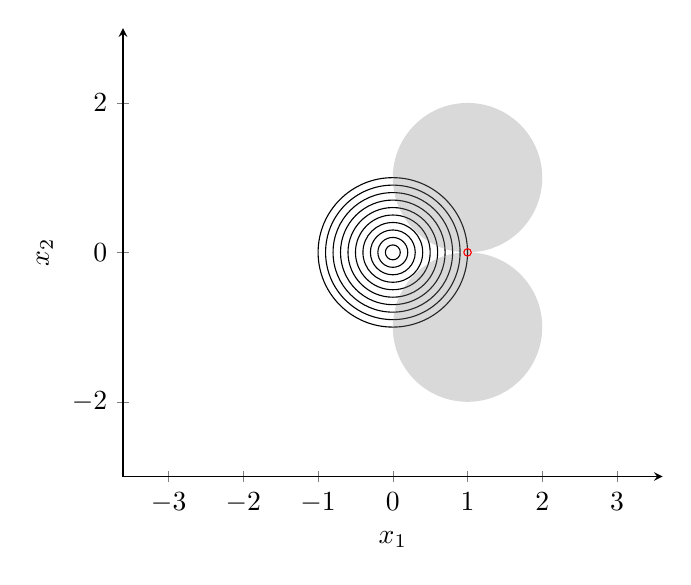
\begin{tikzpicture}
		\begin{axis}[
		axis lines = left,
		xmin=-3, xmax=3, ymin=-3, ymax=3,
		axis equal,
		xlabel = $x_1$,
		ylabel = {$x_2$},
		]
		\draw (axis cs: 0, 0) circle [radius=1];
		\draw (axis cs: 0, 0) circle [radius=.9];
		\draw (axis cs: 0, 0) circle [radius=.8];
		\draw (axis cs: 0, 0) circle [radius=.7];
		\draw (axis cs: 0, 0) circle [radius=.6];
		\draw (axis cs: 0, 0) circle [radius=.5];
		\draw (axis cs: 0, 0) circle [radius=.4];
		\draw (axis cs: 0, 0) circle [radius=.3];
		\draw (axis cs: 0, 0) circle [radius=.2];
		\draw (axis cs: 0, 0) circle [radius=.1];
		\fill [gray, opacity=0.3] (axis cs: 1, -1) circle [radius=1];
		\fill [gray, opacity=0.3] (axis cs: 1, 1) circle [radius=1];
		\draw [red] (axis cs: 1, 0) circle [radius=0.05];
		\end{axis}
	\end{tikzpicture}
	\caption{Level curve, constraints and feasible set}
\end{figure}
\subsubsection*{(b)}
\paragraph{}
The KKT conditions are:
\begin{enumerate}
	\item $(x_1 -1)^2+(x_2-1)^2 \leq 1$, $(x_1 -1)^2+(x_2+1)^2 \leq 1$,
	\item $\lambda_1, \lambda_2 \geq 0 $,
	\item $\lambda_1((x_1 -1)^2+(x_2-1)^2 -1) = 0$, $\lambda_2((x_1 -1)^2+(x_2+1)^2 -1)=0$,
	\item $(1+\lambda_1+\lambda_2)x_1^2 -2(\lambda_1+\lambda_2)x_1 = 0$, $(1+\lambda_1+\lambda_2)x_2^2 -2(\lambda_1-\lambda_2)x_2 = 0$,
\end{enumerate}
\paragraph{}
where (4) is followed by convex problem. Plug in $(1, 0)$ and we have
\begin{align*}
\lambda_1 = 0; \qquad \lambda_2 = 0;\qquad \lambda_1 +\lambda_2 = 1.
\end{align*}
\paragraph{}
Therefore, there is no solution.
\subsubsection*{(c)}
The Lagrangian is
\begin{align*}
&L(x_1, x_2, \lambda_1, \lambda_2) =x_1^2 +x_2^2 +\lambda_1(x_1^2 +x_2^2 -2x_1 -2x_2 +1)\\
&\qquad \qquad \qquad \ \ + \lambda_2(x_1^2 +x_2^2 -2x_1 +2x_2 +1)
\end{align*}
\paragraph{}
Taking partial over $x_1$ and $x_2$ and we have
\begin{align*}
&x_1 = \frac{\lambda_1 +\lambda_2}{1+\lambda_1+\lambda_2}\\
&x_2 = \frac{\lambda_1 -\lambda_2}{1+\lambda_1+\lambda_2}
\end{align*}
\paragraph{}
Since $\lambda_1, \lambda_2 \geq 0$, we always have$1+\lambda_1+\lambda_2 \geq 1$, The dual is therefore given by:
\begin{align*}
&maximize \qquad \frac{-\lambda_1^2 -\lambda_2^2+2\lambda_1 \lambda_2+\lambda_1+\lambda_2}{1+\lambda_1+\lambda_2}\\
&subject\ to \qquad \lambda_1, \lambda_2 \geq 0
\end{align*}
\paragraph{}
Since $g(\lambda_1,\lambda_2)$ is symmetric, the optimum occurs at $\lambda_1 =\lambda_2$, and therefore we have
\begin{align*}
g(\lambda_1) = \frac{2\lambda_1}{1+2\lambda_1}
\end{align*}
\paragraph{}
$g(\lambda_1) = 1$ as $\lambda_1 \rightarrow \infty$, i.e., $p^\star = d^\star$. However, the dual is not attained. 